\documentclass[serif,mathserif,final]{beamer}
\mode<presentation>{\usetheme{Lankton}}

\RequirePackage{fontawesome5}
\usepackage[
  orientation=landscape,
  width=48in,height=36in,%size=a0, % paper size
  scale=1.2 % font scale factor
  ]{beamerposter}
 \setbeamertemplate{caption}[numbered] % number figs

% Graphics Path
\usepackage{graphicx}
\graphicspath{{../../plots/}{./}{../../tikz/}}
\usepackage[%
    %font={footnotesize},
    labelfont=bf,
    format=plain,
    margin=0pt,
]{caption}
\usepackage[list=true]{subcaption}

\usepackage[ttscale=0.8]{libertine} % better font

% OTHER PACKAGE CALLS
\usepackage[utf8]{inputenc}
\usepackage{
  amsmath,
  amsfonts,
  amssymb,
  xspace,
  framed,
  siunitx,
  nth,
  physics,
  nicefrac,
}
%\sisetup{round-mode = figures, round-precision = 3}
\usepackage{cleveref}

%------ BIBLATEX WITH EXTREMELY MINAMALIST STYLE -----
\usepackage[backend=biber,style=nature,maxnames=1,uniquelist=false,date=year]{biblatex}
\ExecuteBibliographyOptions{isbn=false,url=false,doi=false,eprint=false}

% One-paragraph bibliography environment
\defbibenvironment{bibliography}
  {\list
     {\printtext[labelnumberwidth]{%
        \printfield{prefixnumber}%
        \printfield{labelnumber}}%
      \ifentrytype{article}{% Suppress remaining fields/names/lists here
        \clearfield{title}}{}}
     {\setlength{\leftmargin}{0pt}%
      \setlength{\topsep}{0pt}}%
      \renewcommand*{\makelabel}[1]{##1}}
  {\endlist}
  {\mkbibitem}

% \mkbibitem just prints item label and non-breakable space
\makeatletter
\newcommand{\mkbibitem}{\@itemlabel\addnbspace}
\makeatother

% Add breakable space between bibliography items
\renewcommand*{\finentrypunct}{\addperiod\space}

% et al. string upright (nature style applies \mkbibemph)
\renewbibmacro*{name:andothers}{%
  \ifboolexpr{
    test {\ifnumequal{\value{listcount}}{\value{liststop}}}
    and
    test \ifmorenames
  }
    {\ifnumgreater{\value{liststop}}{1}{\finalandcomma}{}%
     \andothersdelim
     \bibstring{andothers}}
    {}}

% Set fields to clear
\AtEveryBibitem{%
	\clearfield{month}%
	\clearfield{day}%
  \clearfield{year}%
  \clearfield{url}%
  \clearlist {language}% this has to be clear list.....
  \clearfield{pages}%
	\clearfield{pagetotal}%
	\clearfield{eprinttype}%
	\clearfield{eprint}%
	\clearfield{number}%
	\clearfield{volume}%
	\clearfield{issue}%
	\clearfield{name:given}
	\clearfield{name:first}
	\ifentrytype{article}{%
		\clearfield{title}%
	}%
}

\addbibresource{library.bib}

%------- GLOSSARIES PACKAGE -------
\usepackage[acronym]{glossaries}
\newacronym{rcp}{RCP}{representative concentration pathway}
\newacronym[]{fema}{FEMA}{the Federal Emergency Management Agency}
\newacronym{bfe}{BFE}{base flood elevation}

\usepackage{xspace}
\makeatletter
\DeclareRobustCommand\onedot{\futurelet\@let@token\@onedot}
\def\@onedot{\ifx\@let@token.\else.\null\fi\xspace}
\def\eg{\emph{e.g}\onedot} \def\Eg{\emph{E.g}\onedot}
\def\ie{\emph{i.e}\onedot} \def\Ie{\emph{I.e}\onedot}
\def\etc{\emph{etc}\onedot} \def\vs{\emph{vs}\onedot}

%-- Header and footer information ----------------------------------
\newcommand{\footleft}{\textbf{Preprint Coming Soon}: follow \href{https://twitter.com/jdossgollin}{@jdossgollin} on Twitter or visit \href{https://dossgollin-lab.github.io}{dossgollin-lab.github.io}}
\newcommand{\footright}{\textbf{Let's Collaborate!} \href{mailto:jdossgollin@rice.edu}{jdossgollin@rice.edu}}
\title{Which Scenario Should We Design For? Insights from House Elevation for the Multiple PDF Problem}
\author{James Doss-Gollin\inst{*1} \quad Klaus Keller\inst{2,3,4}}
\institute{\inst{*}\href{mailto:jdossgollin@rice.edu}{jdossgollin@rice.edu} \quad \inst{1} Department of Civil and Environmental Engineering, Rice University \\  \inst{2} Department of Geosciences, the Pennsylvania State University \quad \inst{3} Earth and Environmental Systems Institute, the Pennsylvania State University \quad \inst{4} Thayer School of Engineering, btmouth College}

%-------------------------------------------------------------------


%-- Main Document --------------------------------------------------
\begin{document}
\begin{frame}{}
  \begin{columns}[t]

    %-- Column 1 ---------------------------------------------------
    \begin{column}{0.22\linewidth}

      \begin{block}{house elevation}
    Households elevate their homes to manage flood risks, but regulations and guidance are silent on key questions \cite{zarekarizi_suboptimal:2020,xian_elevation:2017}.
    \vspace*{-1em}
    \begin{description}
        \item[Q1] How to adapt guidance to building characteristics or household preferences?
        \item[Q2] How does nonstationary hazard change guidance?
        \item[Q3] Which model of nonstationary hazard to use?
    \end{description}
    \begin{framed}
        \begin{figure}
            \centering
            \subcaptionbox{Selinsgrove, PA}{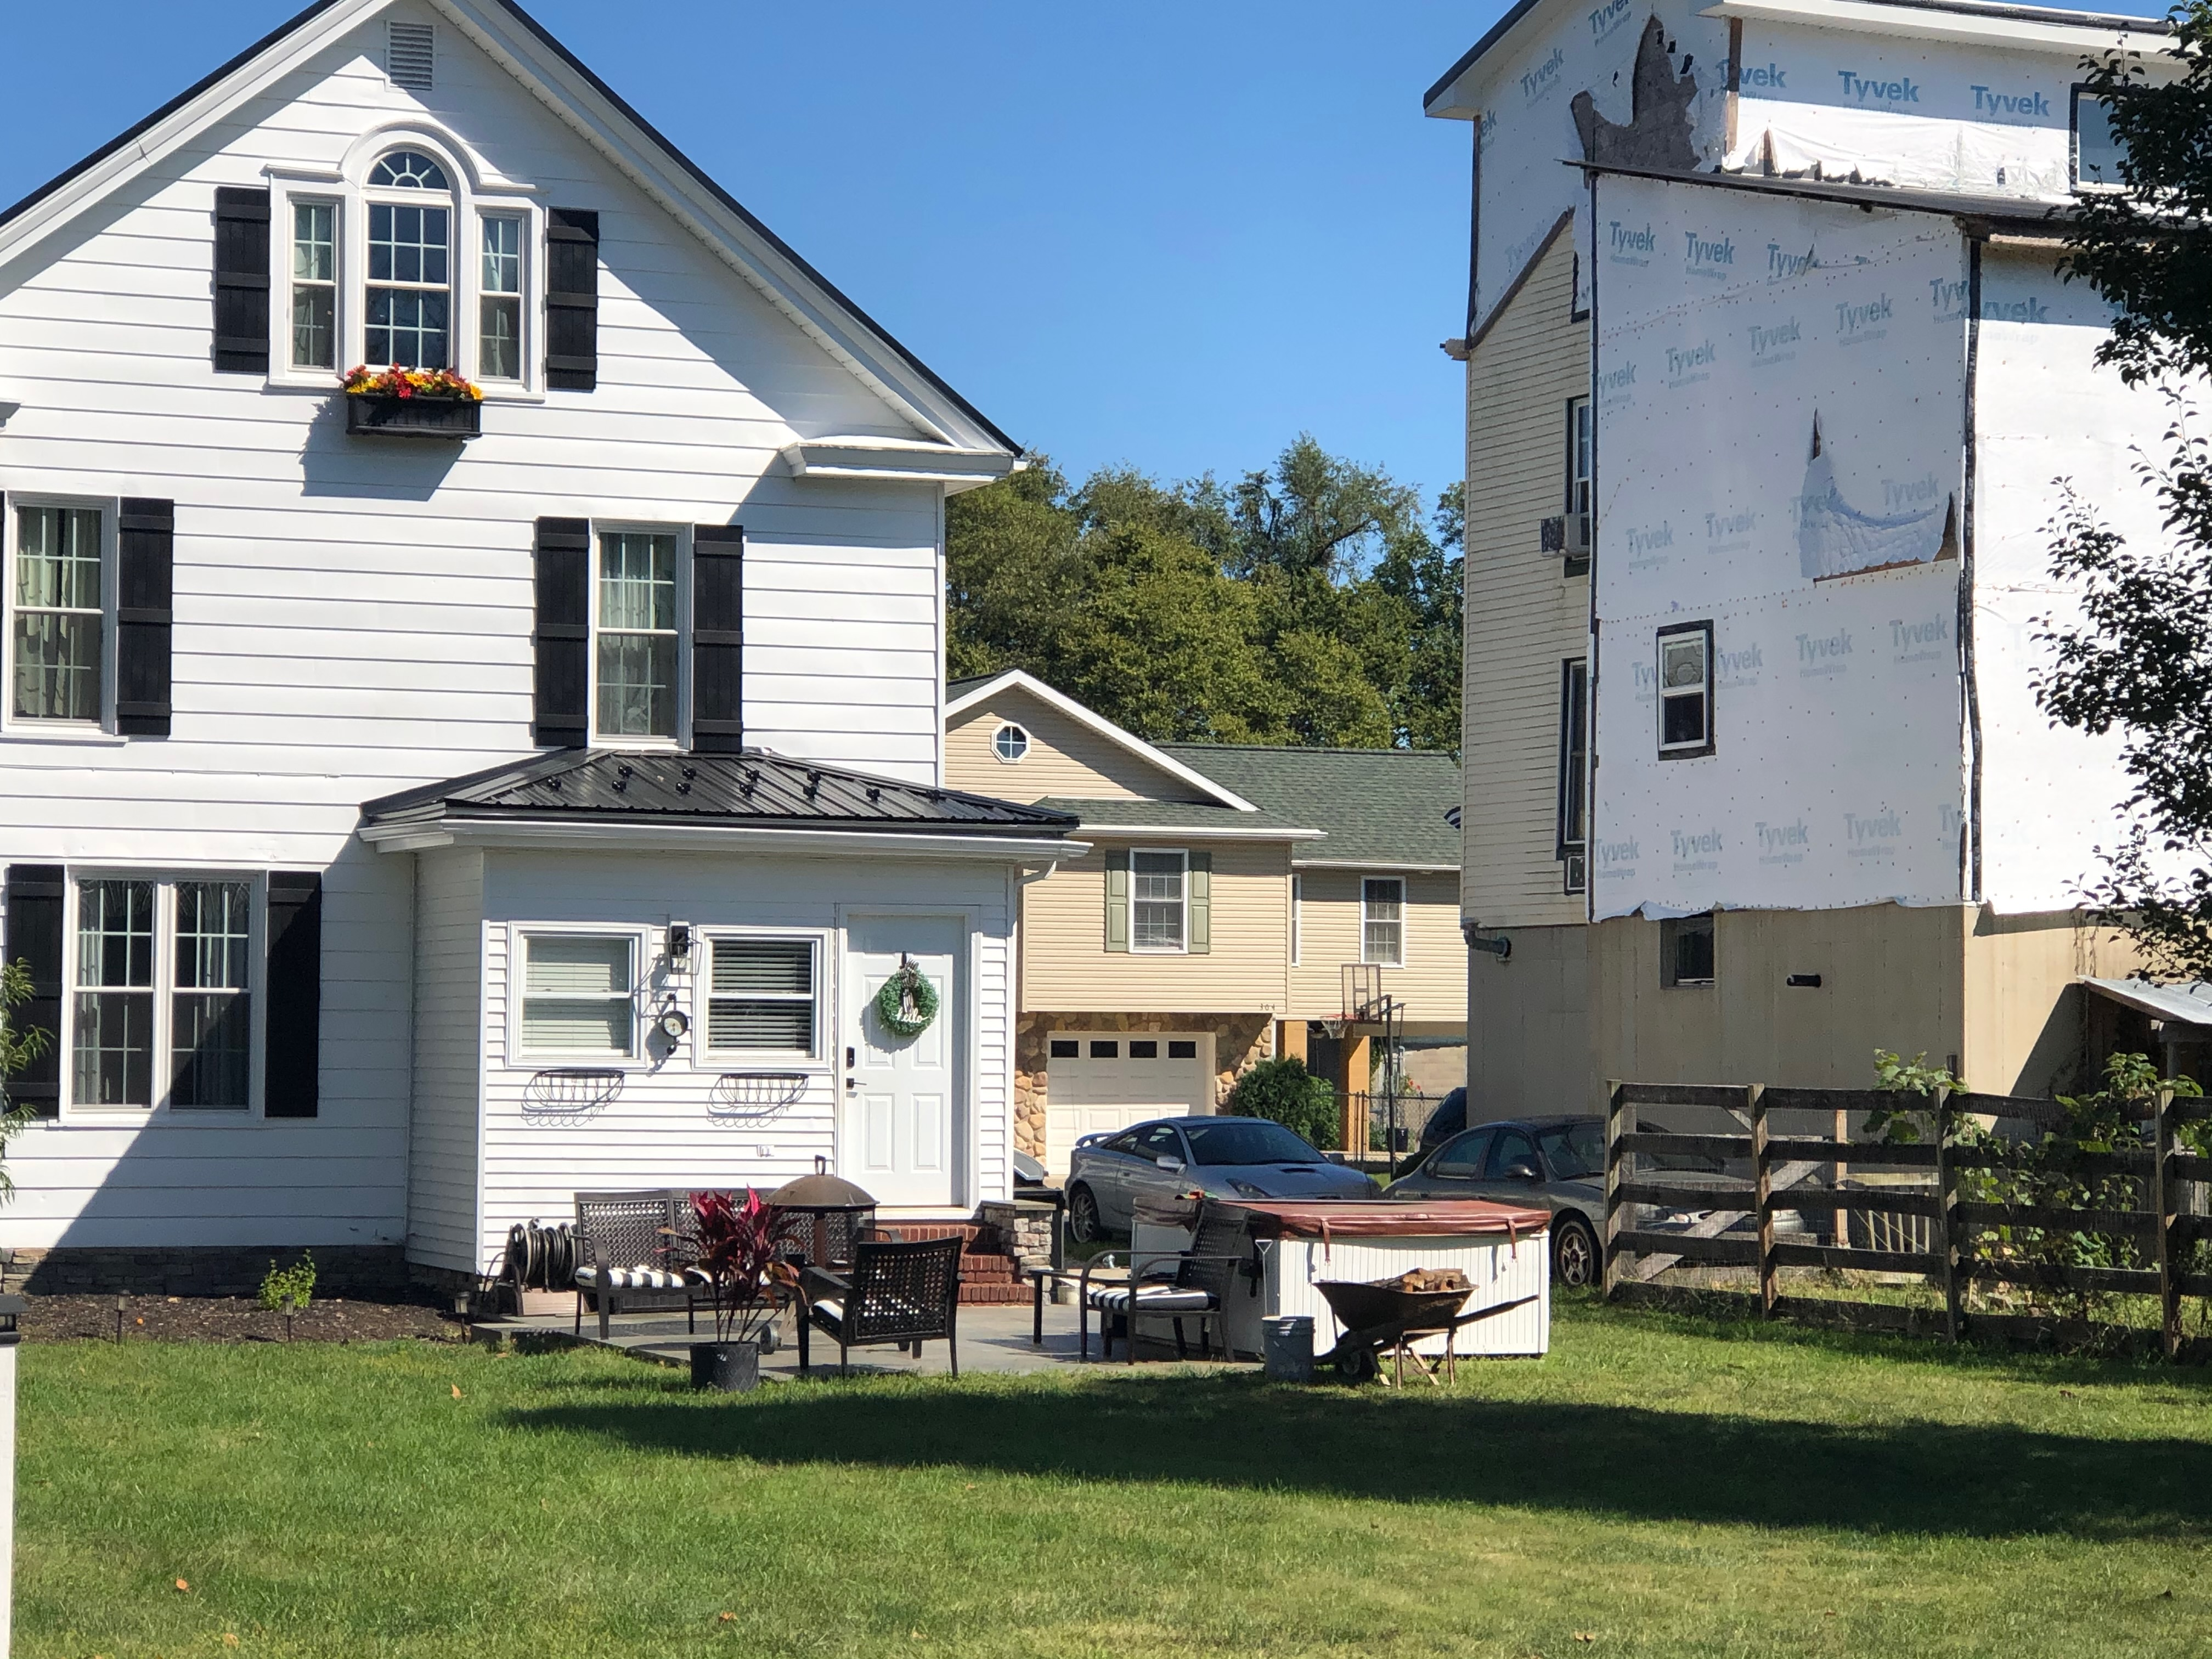
\includegraphics[height=3.35in]{img_selinsgrove.jpeg}}%
            \hfill%
            \subcaptionbox{Houston, TX}{\includegraphics[height=3.35in]{img_braeswood.png}}\\
            \subcaptionbox{Plaquemines Parish, LA}{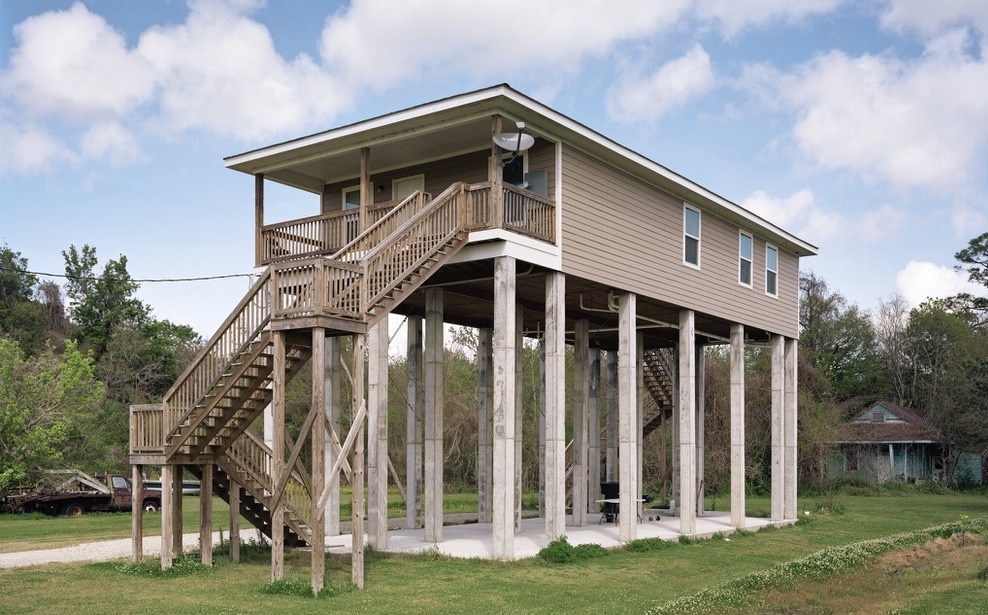
\includegraphics[height=3.3in]{epstein-2020-la.jpeg}}%
            \hfill%
            \subcaptionbox{Dare County, NC}{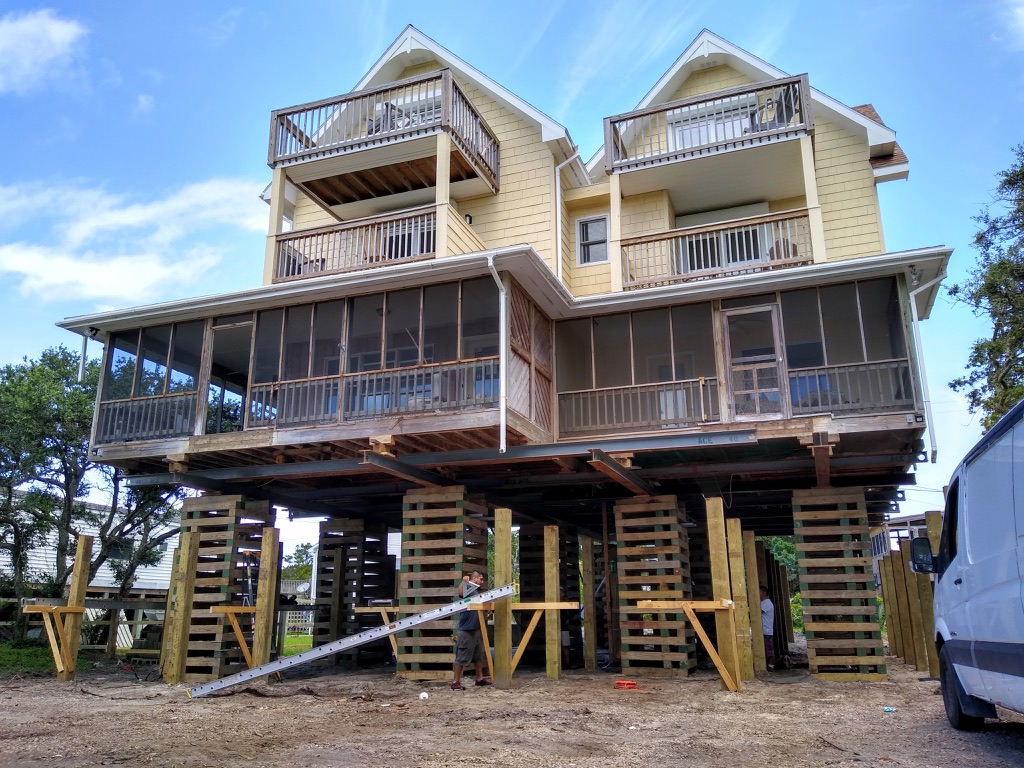
\includegraphics[height=3.3in]{nichols-ocracoke.jpeg}}%
            \caption{
                \faIcon{camera}: (a) JDG, (b) Google Maps, (c) Mitch Epstein /  New York Times (d) Rob Nichols / PSU.
            }
            \label{fig:images}
        \end{figure}
    \end{framed}
    These challenges also affect other adaptation plans and engineering designs (\cref{fig:stormwater-bridge}).
\end{block}
      \begin{block}{case study: norfolk, va}
    We model a \emph{hypothetical} house in Norfolk, VA, where sea level rise drives nonstationary future flood hazard, following the approach of \cite{zarekarizi_suboptimal:2020}.
    \begin{figure}
        \centering
        \includegraphics[width=\textwidth]{historic_surge.pdf}
        \caption{
            Time series of annual maximum of storm surge (after subtracting mean sea level) at Sewells Point, VA (NAVD datum).
        }
        \label{fig:observations}
    \end{figure}
    \begin{figure}
        \centering
        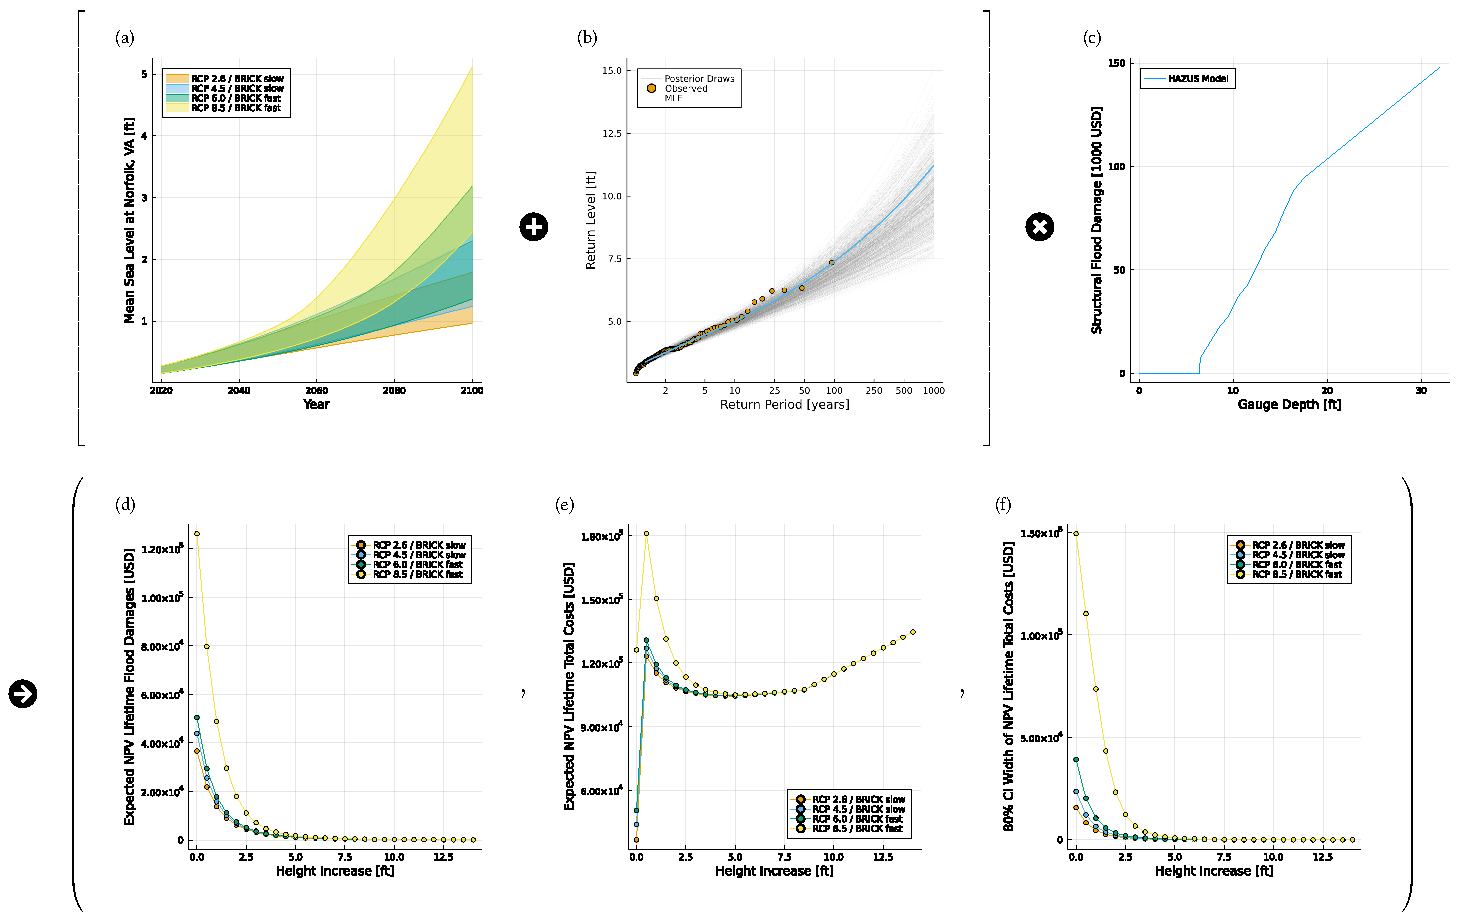
\includegraphics[width=\textwidth]{hazard-tradeoffs.pdf}
        \caption{
            Neglecting hydrodynamics, we add sea level rise (a; see ref.~\cite{ruckert_coastal:2019}) to a Bayesian GEV model of storm surge (b) to get flood hazard.
            The convolution of hazard and fragility (c; see ref.~\cite{zarekarizi_suboptimal:2020}) yields an assessment of damages and tradeoffs (\cref{fig:tradeoffs}).
        }
    \end{figure}
\end{block}

    \end{column}%1

    %-- Column 2 ---------------------------------------------------
    \begin{column}{0.22\linewidth}

      \begin{block}{one size doesn't fit all!}
    \begin{itemize}
        \item Tailoring guidance to specific building characteristics can improve outcomes
        \item Elevating to ``\gls{bfe} plus a foot'' is not always optimal \cite{xian_elevation:2017,zarekarizi_suboptimal:2020}
        \item Both over- and under-building can be costly \cite{ansar_bigisfragile:2017,DossGollin:2019}
    \end{itemize}
    \begin{framed}
        \begin{figure}
            \centering
            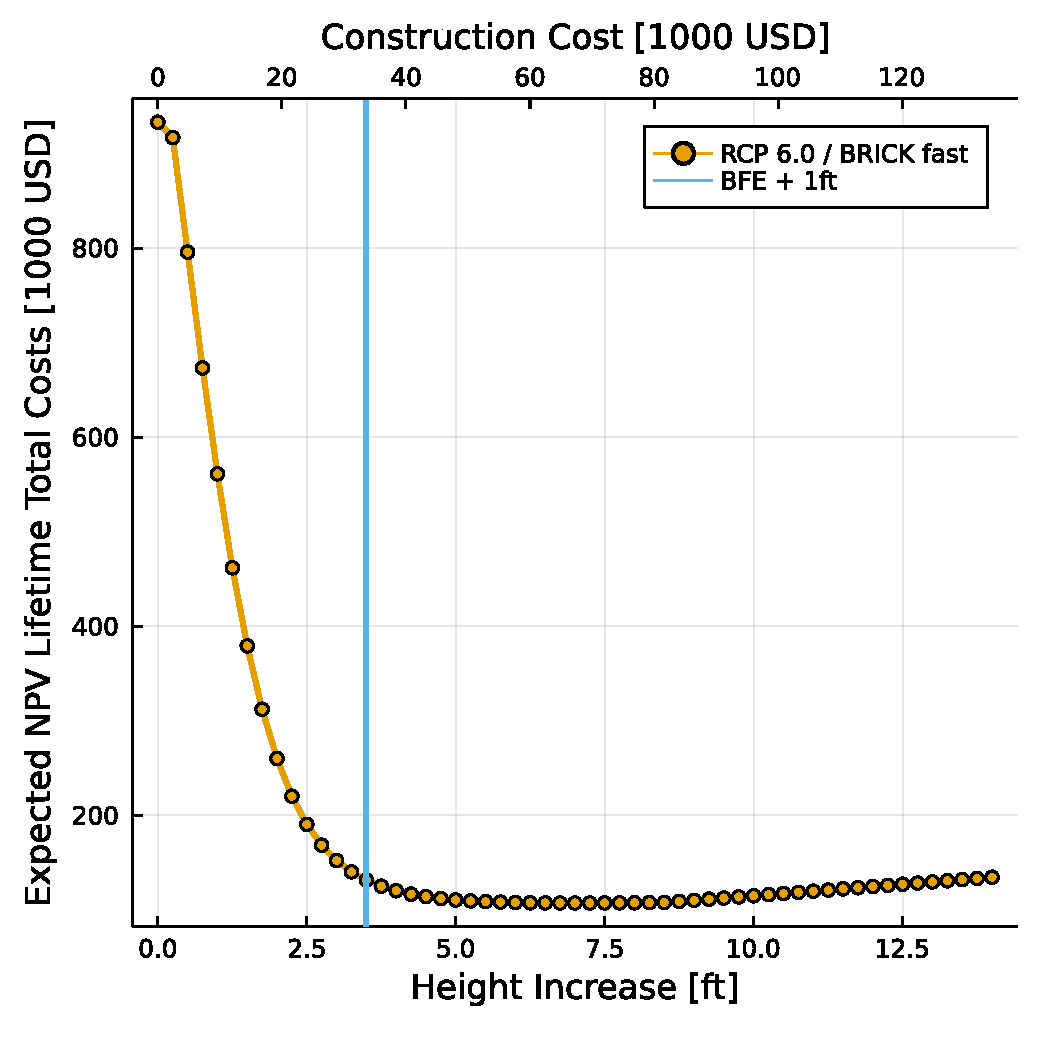
\includegraphics[width=0.475\textwidth]{5.5.pdf}%
            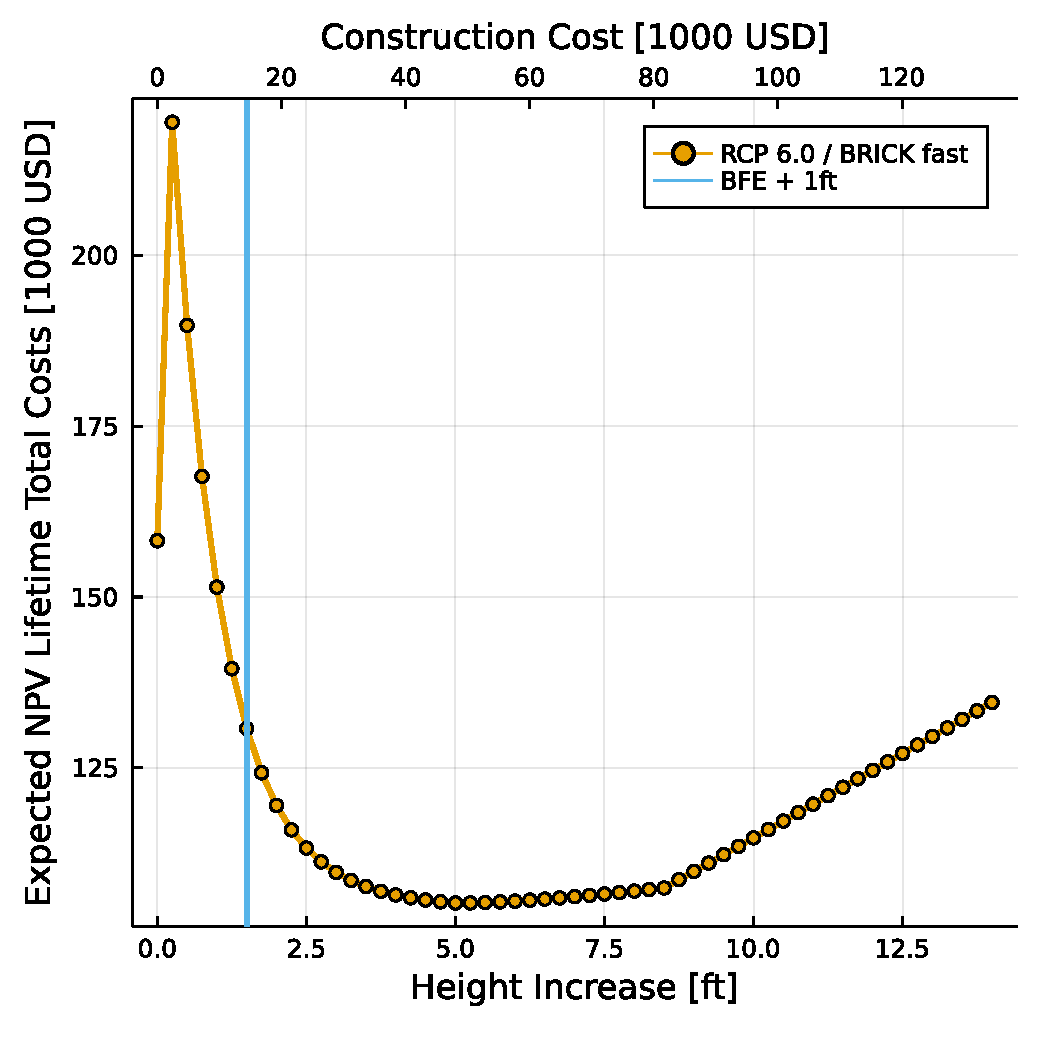
\includegraphics[width=0.475\textwidth]{7.5.pdf}
            \caption{
                Tradeoffs between construction cost and expected NPV lifetime costs for houses initially situated (L) \SI{2.5}{ft} and (R) \SI{0.5}{ft} below the \gls{bfe} under \gls{rcp} 6.0 with fast BRICK dynamics.
                Note $y$-axes are not equal.
            }
        \end{figure}
    \end{framed}
\end{block}
      \begin{block}{the multiple pdf problem}
    Uncertainties from multiple model structures (\eg, ice sheet dynamics) and/or scenarios (\eg, emissions pathways) create multiple estimates of time-varing hazard, \ie, the \textbf{\itshape{Multiple PDF Problem}}.
    Including additional models \cite{kopp_evolving:2017,deconto_antarctica:2016,ruckert_coastal:2019} \emph{would compound this challenge}.
    \begin{framed}
        \begin{figure}
            \centering
            \includegraphics[width=\textwidth]{msl_boxplots.pdf}
            \caption{
                Sea level rise projections use the BRICK model \cite{wong_brick0.2:2017,ruckert_coastal:2019}.
                We consider \emph{eight time-dependent PDFs of sea level rise}: four \gls{rcp} scenarios $\times$ two parameterizations of ice sheet processes.
            }\label{fig:boxplots}
        \end{figure}
    \end{framed}
\end{block}
      \begin{block}{references}
        \renewcommand*{\bibfont}{\footnotesize}
        \printbibliography[heading=none]
      \end{block}

    \end{column}

    %-- Column 3 ---------------------------------------------------
    \begin{column}{0.22\linewidth}

      \begin{block}{it matters which pdf you choose!}
    Any optimal strategy or Pareto frontier is conditional upon an (explicit or implicit) model of future outcomes (see ref.~\cite{gelman_philosophy:2013} for a more philosophical discussion).
    \begin{framed}
        \begin{figure}
            \centering
            \includegraphics[width=0.48\textwidth]{tradeoffs_height_totalcost_byscenario.pdf}%
            \includegraphics[width=0.48\textwidth]{tradeoffs_height_iqr_byscenario.pdf}
            \caption{
                Tradeoffs between (L) construction cost and expected lifetime costs or (R) construction cost and the uncertainty of future lifetime costs depend on the model selected.
            }
            \label{fig:tradeoffs}
        \end{figure}
    \end{framed}
    Weights assigned to PDFs or simulations, \textbf{including implicit uniform weights}, should be communicated transparently to facilitate critique and improvement
\end{block}
      \begin{block}{synthesizing pdfs for decision relevance}
    If there are only a few PDFs, then qualitative comparisions (\eg, \cref{fig:tradeoffs}) may be sufficient.
    With \emph{many} PDFs (\eg, \cref{fig:boxplots}), further synthesis is needed.

    We consider the \emph{common case} of assessing decisions using simulations (SOWs) from each of $K$ PDFs.
    \begin{figure}
        \centering
        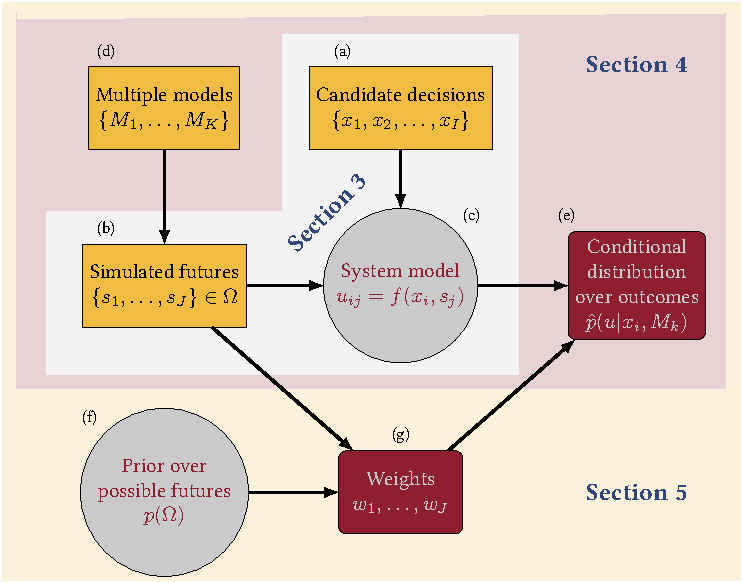
\includegraphics[width=\textwidth]{bayes-rdm.pdf}
        \caption{
            Sketch of the ``Prior Model Averaging'' framework.
        }\label{fig:flowchart}
    \end{figure}
\end{block}


    \end{column}

    %-- Column 4 ---------------------------------------------------
    \begin{column}{0.22\linewidth}

      \begin{block}{different beliefs emphasizes different possibilities}
    The prior model averaging approach (\cref{fig:flowchart}) assigns a weight to each PDF based on their
    \begin{itemize}
        \item The prior can't be ``right''  \cite{gelman_workflow:2020,gelman_philosophy:2013} or ``scenario neutral'' \cite{quinn_exploratory:2020}
        \item let's at least \textbf{make assumptions transparent}!
    \end{itemize}
    \begin{figure}
        \centering
        \includegraphics[width=\textwidth]{lsl_priors.pdf}
        \caption{
            If we weight all scenarios equally, then our projection of MSL in 2100 follows the sampling distribution; this may or may not reflect available information.        }
    \end{figure}
    \begin{figure}
        \centering
        \includegraphics[width=\textwidth]{inference_weights.pdf}
        \caption{
            Weights assigned to each PDF (from \cref{fig:boxplots}) under each prior considered.
            Horizontal line shows the weight given to each under an implicit uniform assumption.
        }
    \end{figure}
\end{block}
      \begin{block}{looking ahead}
    This didactic example illustrates a need for better synthesis and communication of deep uncertainties for decision making.
    \textbf{\scshape let's collaborate on:}
    \begin{itemize}
        \item More complex models to capture more relevant metrics
        \item Better priors over nonstationary hazard
        \item Interacting, sequential decisions
        \item Inclusive assessment of ethical questions around scenario weighting
    \end{itemize}
    \begin{framed}
        \begin{figure}
            \centering
            \subcaptionbox{Stormwater}{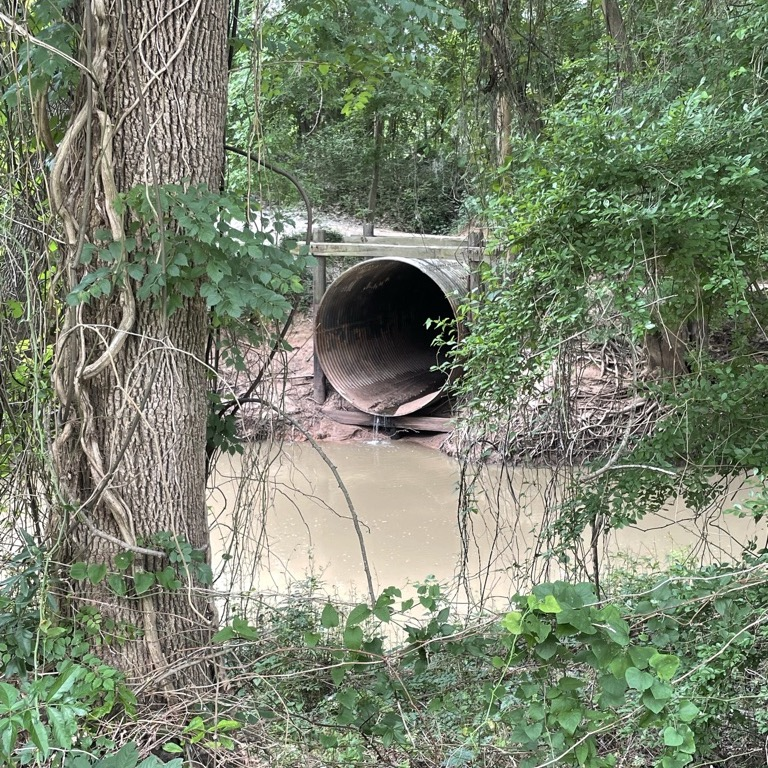
\includegraphics[height=3.5in]{culvert.jpeg}}%
            \hfill
            \subcaptionbox{Bridge Clearance}{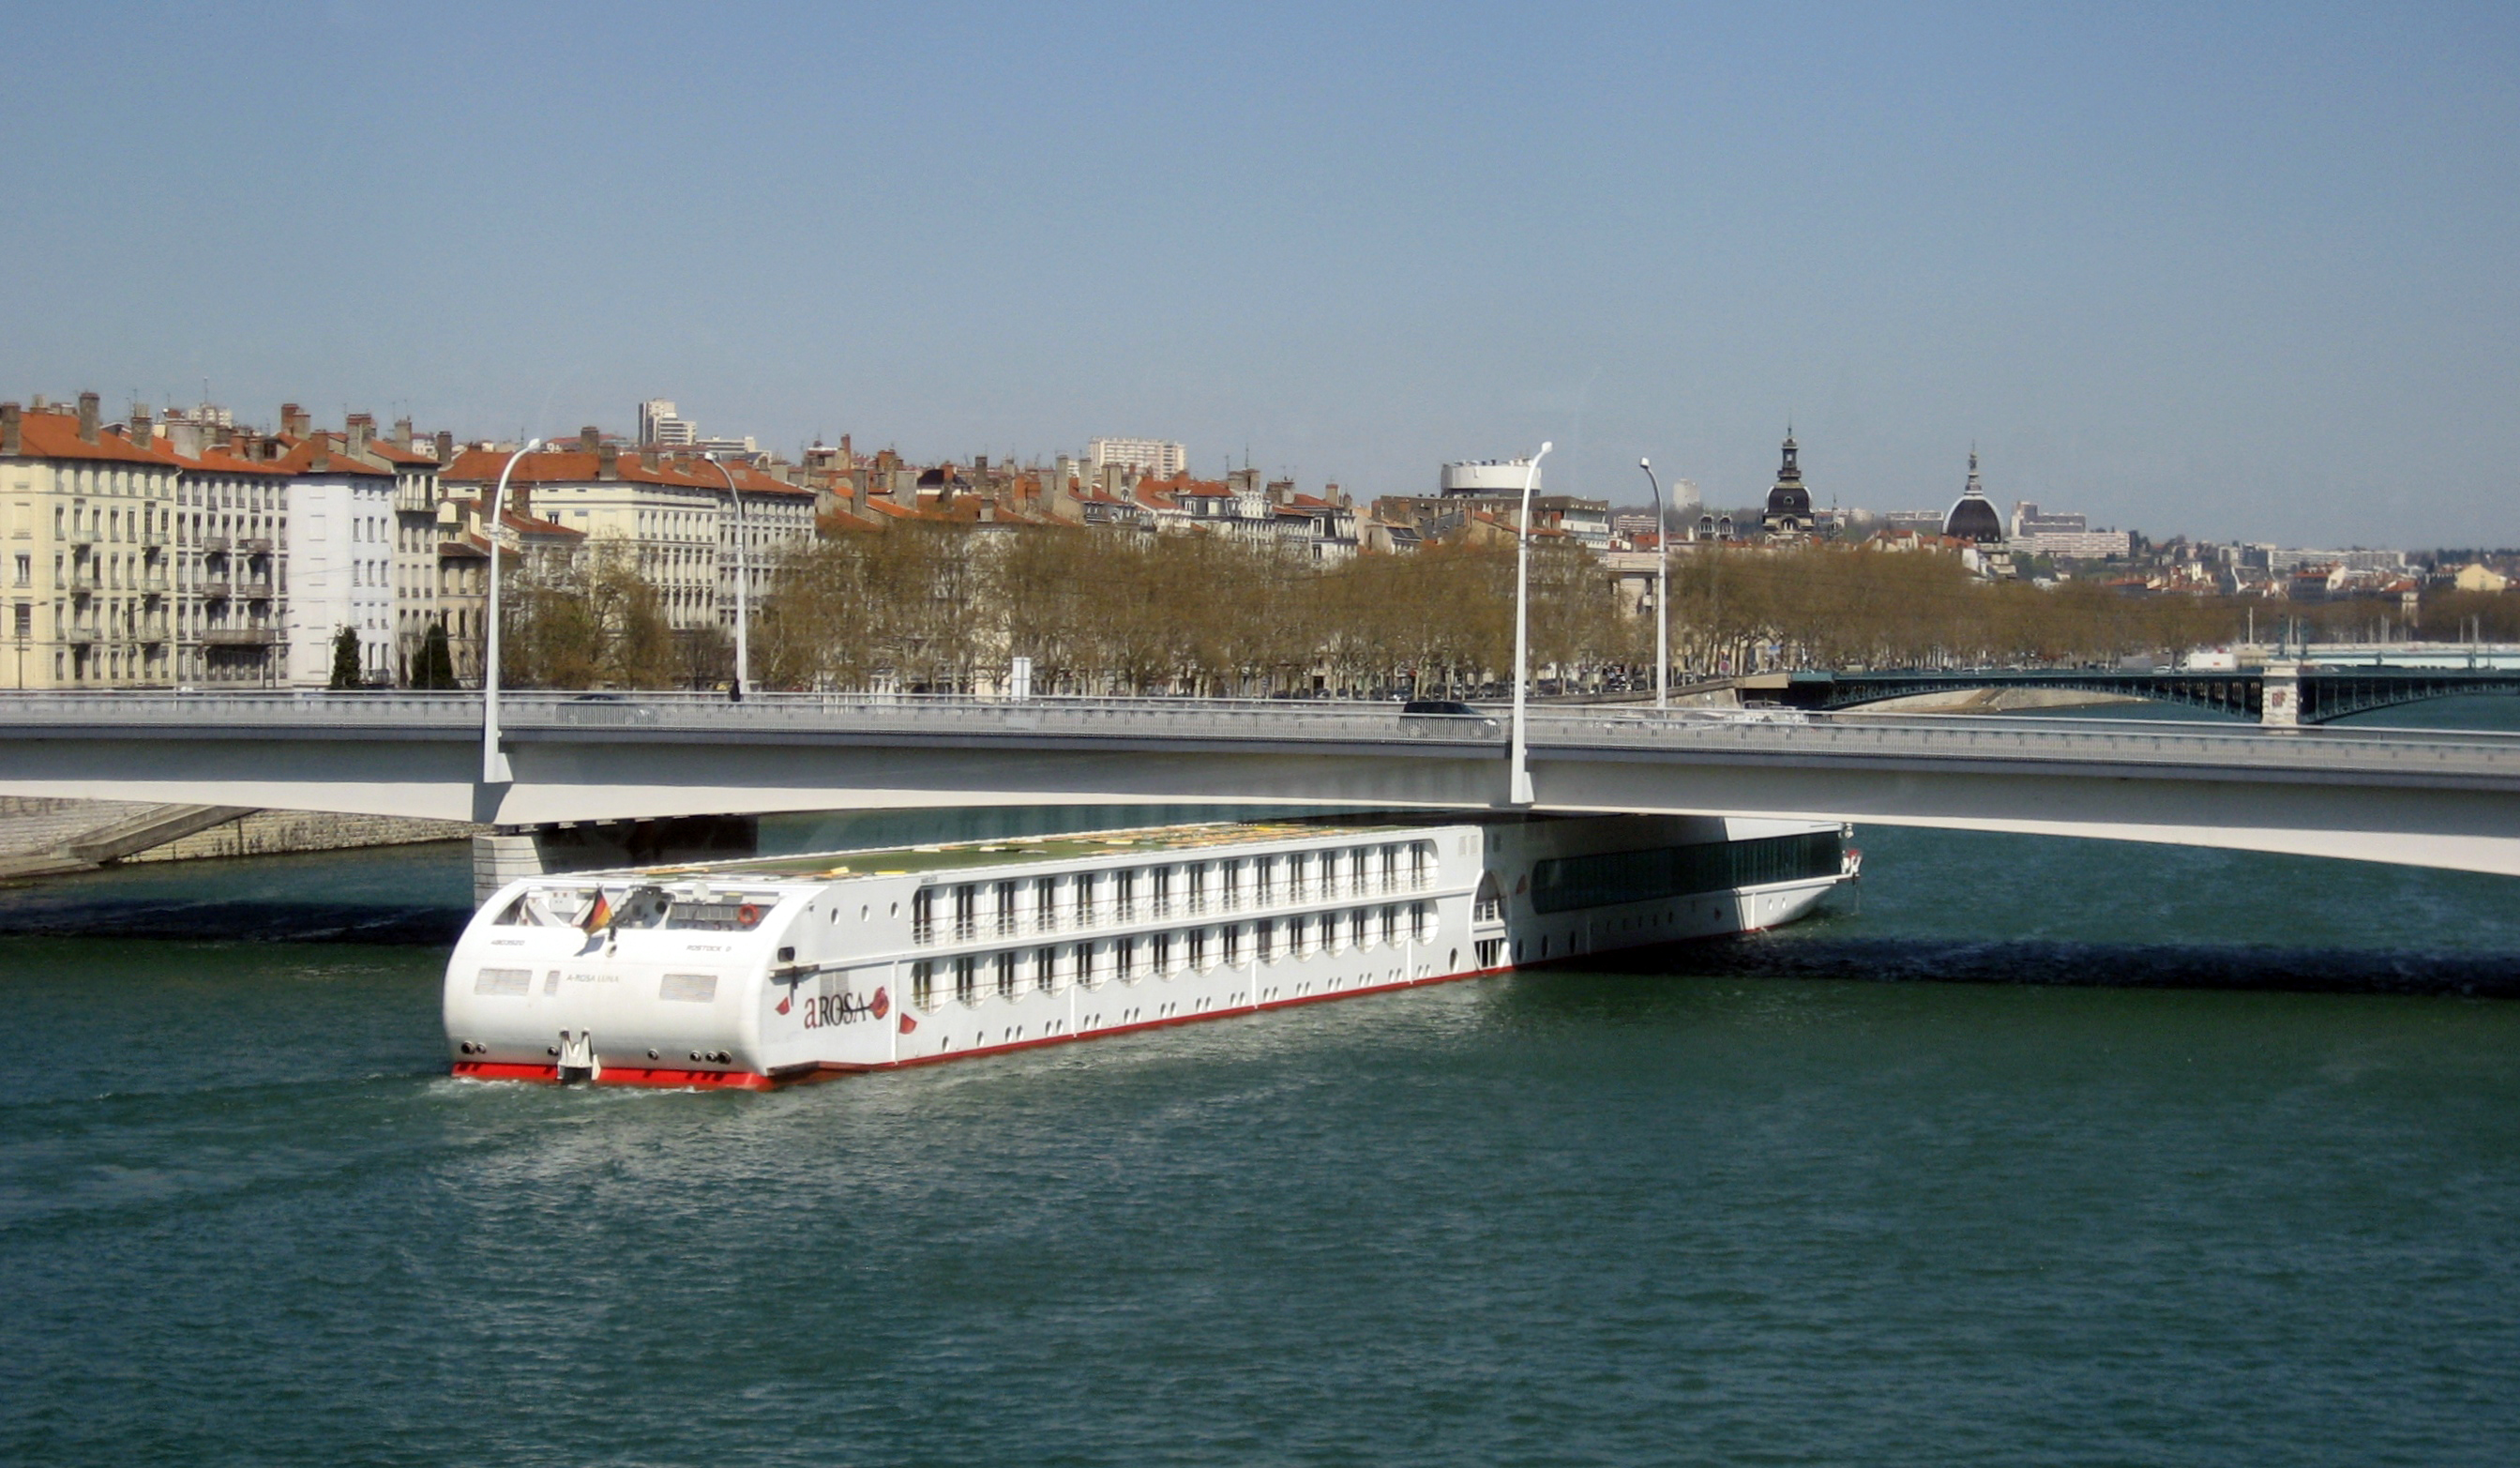
\includegraphics[height=3.5in]{bridge_clearance.jpg}}
            \caption{
                House elevation is just one of many design problems where nonstationary hazards, subject to scenario and model structure uncertainties, drive outcomes.
                \faIcon{camera}: (a) JDG (b) D. Howard / Wikipedia.
            }
            \label{fig:images}
        \end{figure}
    \end{framed}
\end{block}

    \end{column}
  \end{columns}
\end{frame}
\end{document}
